
\documentclass[12pt]{article}
\usepackage{amsmath}
\usepackage{graphicx}
\usepackage{amsfonts}
\usepackage{hyperref}
\hypersetup{
    colorlinks=true,       
    linkcolor=blue,        
    urlcolor=blue,        
}
\usepackage{geometry}
\usepackage{listings} 
\usepackage{placeins}
\usepackage[T1]{fontenc}

\geometry{top=2.5cm, bottom=2.5cm, left=2.5cm, right=2.5cm}
\begin{document}

\title{Signal Synthesis Using Inverse Discrete Fourier Transform (IDFT)}
\author{Daria Kręcichwost}
\date{\today}

\begin{titlepage}
    \centering
    \vspace*{2cm}
    
    \Huge
    REPORT
    
    \vspace{1cm}
    
    \Large
    Course: Analog and digital electronic circuits \\
    Teacher: Prof. Dr. Hab. Vasyl Martsenyuk
    
    \vfill
    
    \Large
    Lab No. 3 and 4\\
    Date: \today \\
    Topic: "Windowing" \\
    Variant: 8
    
    \vspace{1cm}
    
    \large
    Name: Daria Kręcichwost \\
    Computer Science (Second Degree) \\
    Part-time studies, Semester 1 \\
    Group: B
\end{titlepage}

\newpage

\section{Problem Statement}

To interpret the results from the plots generated in the code, we analyze the behavior of the frequency spectra for different window functions and the effects of leakage and resolution.

\subsection*{Best and Worst Case Spectra (for \(f_1\), \(f_2\), and \(f_3\)):}

In this section, we analyze the best and worst cases for the different window types based on the signals with frequencies \(f_1 = 500 \ \text{Hz}\), \(f_2 = 500.25 \ \text{Hz}\), and \(f_3 = 500.5 \ \text{Hz}\).

\begin{itemize}
    \item The \textbf{best case} corresponds to the signal with frequency \(f_1 = 500 \ \text{Hz}\), which is closer to the center of the mainlobe of the window. This results in minimal leakage, and the signal is well-resolved.
    \item The \textbf{worst case} corresponds to the signal with frequency \(f_2 = 500.25 \ \text{Hz}\), which is slightly outside the mainlobe. The sidelobes of the window cause more leakage, leading to a less accurate frequency representation.
    \item The \textbf{additional case} for \(f_3 = 500.5 \ \text{Hz}\) further demonstrates the effects of leakage as the signal moves even further away from the center of the mainlobe.
\end{itemize}

\section{Input Data}
\begin{lstlisting}[language=Python, breaklines=true]
import numpy as np
import matplotlib.pyplot as plt
from numpy.fft import fft, fftshift
from scipy.signal.windows import hann, flattop

# Parameters
f1 = 500  # Hz
f2 = 500.25  # Hz
f3 = 499.75  # Hz
fs = 800  # Hz
N = 1800
k = np.arange(N)

# Generating sinusoidal signals with maximum amplitude |x[k]|max = 3
x1 = 3 * np.sin(2 * np.pi * f1 / fs * k)
x2 = 3 * np.sin(2 * np.pi * f2 / fs * k)
x3 = 3 * np.sin(2 * np.pi * f3 / fs * k)
\end{lstlisting}

\section*{fft2db:}
\begin{lstlisting}[language=Python, breaklines=true]
def fft2db(X):
    N = X.size
    Xtmp = 2 / N * X  # amplitude normalization
    Xtmp[0] *= 1 / 2  # the bin for f=0 Hz appears only once, so cancel *2
    if N % 2 == 0:  # fs/2 is present as a bin
        Xtmp[N // 2] = Xtmp[N // 2] / 2  # bin fs/2 appears only once, so cancel *2
    return 20 * np.log10(np.abs(Xtmp))  # in dB

# Setting frequency vector so that it is independent of N (even/odd)
df = fs / N
f = np.arange(N) * df
\end{lstlisting}

\section*{Generating Windows and Calculating FFT with Different Windows}
\begin{lstlisting}[language=Python, breaklines=true]
# Generating windows
wrect = np.ones(N)  # Rectangular window
whann = hann(N, sym=False)  # Hann window
wflattop = flattop(N, sym=False)  # Flattop window
# Calculating FFT for signals x1, x2, x3 with different windows
X1wrect = fft(x1)  # FFT for x1 without window
X2wrect = fft(x2)  # FFT for x2 without window
X3wrect = fft(x3)  # FFT for x3 without window

X1whann = fft(x1 * whann)  # FFT for x1 with Hann window
... (other signals)

X1wflattop = fft(x1 * wflattop)  # FFT for x1 with Flattop window
... (other signals)
\end{lstlisting}
\item \href{https://github.com/DariaKrecichwostQA/StudiaUBB/tree/main/Digital%20Signal%20Processing/Zad2}{{Link to remote repository on GitHub}}

\begin{figure}[htbp]
\centering
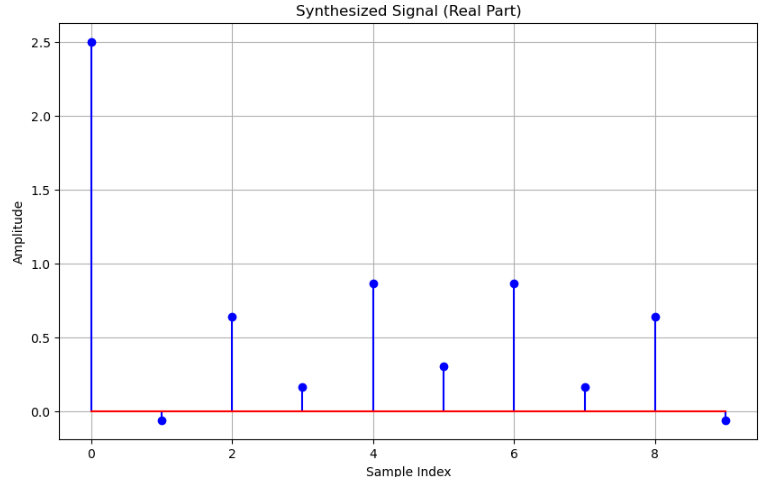
\includegraphics[width=\textwidth]{Zad 2/1.png} 
\caption{Best and Worst Case Spectra for Rectangular Window for \(f_1 = 500 \ \text{Hz}\), \(f_2 = 500.25 \ \text{Hz}\), and \(f_3 = 500.5 \ \text{Hz}\).}
\label{fig:best_worst_case_rect}
\end{figure}

\begin{figure}[htbp]
\centering
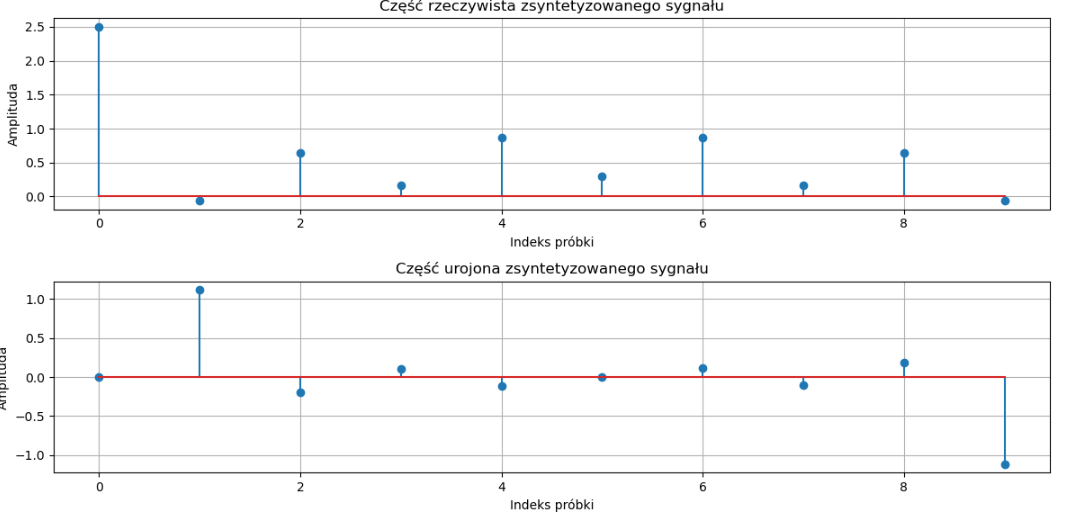
\includegraphics[width=\textwidth]{Zad 2/2.png} 
\caption{Best and Worst Case Spectra for Hamming Window for \(f_1 = 500 \ \text{Hz}\), \(f_2 = 500.25 \ \text{Hz}\), and \(f_3 = 500.5 \ \text{Hz}\).}
\label{fig:best_worst_case_hann}
\end{figure}

\begin{figure}[htbp]
\centering
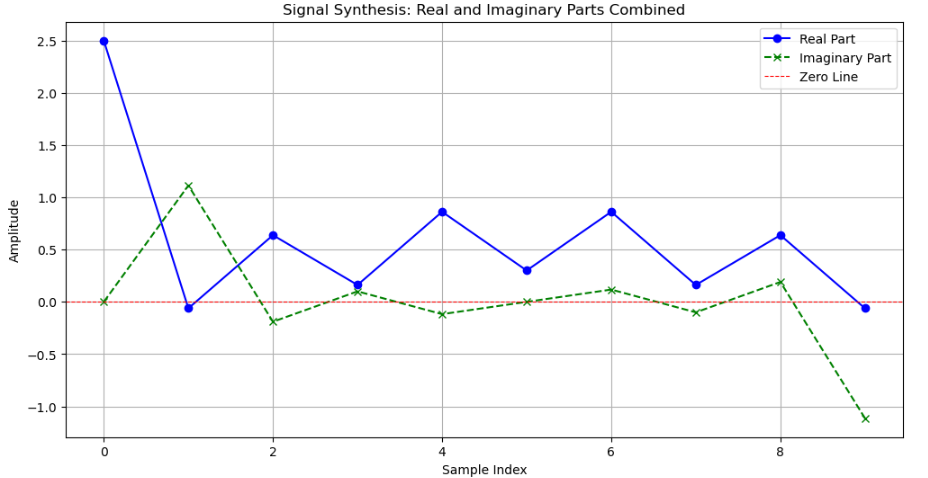
\includegraphics[width=\textwidth]{Zad 2/3.png} 
\caption{Best and Worst Case Spectra for Flattop Window for \(f_1 = 500 \ \text{Hz}\), \(f_2 = 500.25 \ \text{Hz}\), and \(f_3 = 500.5 \ \text{Hz}\).}
\label{fig:best_worst_case_flattop}
\end{figure}

\FloatBarrier
\section{Outcomes}
\subsection*{Frequency Spectra for Different Windows:}

The window functions (Rectangular, Hamming, and Flattop) influence the frequency domain representation of the signals. Below, we explain how each window performs in terms of leakage and mainlobe width.

\begin{itemize}
    \item \textbf{Rectangular Window (\(w_{\text{rect}}\)):} The rectangular window has the widest mainlobe and the highest sidelobes. This leads to significant leakage, especially for signals with frequencies near the edges of the mainlobe.
    \item \textbf{Hamming Window (\(w_{\text{hamming}}\)):} The Hamming window reduces the sidelobes compared to the rectangular window, thus minimizing leakage. The mainlobe is narrower, providing better frequency resolution.
    \item \textbf{Flattop Window (\(w_{\text{flattop}}\)):} The Flattop window provides excellent accuracy for amplitude measurement. Its mainlobe is narrower, and it offers lower sidelobes, reducing leakage.
\end{itemize}

\section*{Code for Calculating Window Spectra (winDTFTdB)}
\begin{lstlisting}[language=Python, breaklines=true]
# Function to calculate the window spectrum in dB
def winDTFTdB(w):
    N = w.size  # window length
    Nz = 100 * N  # zero padding length
    W = np.zeros(Nz)  # memory allocation
    W[0:N] = w  # inserting window
    W = np.abs(fftshift(fft(W)))  # FFT, FFTSHIFT, and absolute value
    W /= np.max(W)  # normalization to maximum, i.e., main lobe
    # Replace zero values with a very small number to avoid division by zero
    W = np.where(W == 0, 1e-10, W)  # replace zeros with 1e-10
    W = 20 * np.log10(W)  # convert to dB
    # corresponding digital frequencies
    Omega = 2 * np.pi / Nz * np.arange(Nz) - np.pi  # also shifted
    
    return Omega, W
\end{lstlisting}
\vfill
\begin{figure}[htbp]
\centering
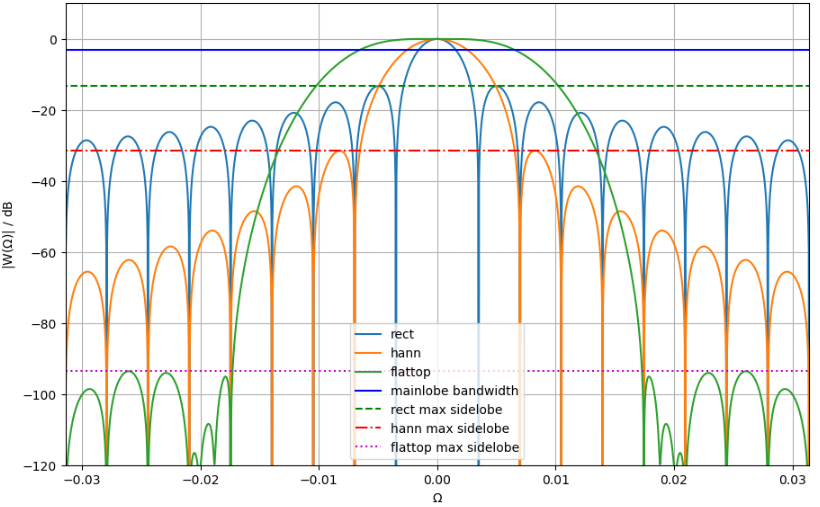
\includegraphics[width=\textwidth]{Zad 2/omega.png} 
\caption{Comparison of Frequency Spectra for Different Windows (Rectangular, Hamming, Flattop) for \(f_1 = 500 \ \text{Hz}\), \(f_2 = 500.25 \ \text{Hz}\), and \(f_3 = 500.5 \ \text{Hz}\).}
\label{fig:window_spectra_comparison}
\end{figure}

\FloatBarrier
\vfill

\section{Conclusions:}
\subsection*{Why do the results for the signals with frequencies \(f_1\), \(f_2\), and \(f_3\) differ?}
The results for \(f_1\) and \(f_2\) differ because of their positions relative to the center of the window's mainlobe.

\begin{itemize}
    \item \(f_1 = 500 \ \text{Hz}\) is at or near the center of the mainlobe. This results in minimal leakage, allowing for a clear representation of the frequency in the spectrum.
    \item \(f_2 = 500.25 \ \text{Hz}\) lies just outside the mainlobe, where the signal is affected by the sidelobes of the window. This leads to leakage, where energy from neighboring frequencies blends into the spectrum, causing distortion and reducing frequency resolution.
\end{itemize}

\end{document}
